\documentclass{article}
\usepackage[margin=1in]{geometry}
\usepackage{amsmath,amsthm,amssymb}
\usepackage{bbm,enumerate,mathtools}
\usepackage{tikz,pgfplots}
\usepackage{chessboard}
\usepackage[hidelinks]{hyperref}
\usepackage{multicol} % Problem 35

\newenvironment{question}{\begin{trivlist}\item[\textbf{Question.}]}{\end{trivlist}}
\newenvironment{note}{\begin{trivlist}\item[\textbf{Note.}]}{\end{trivlist}}
\newenvironment{references}{\begin{trivlist}\item[\textbf{References.}]}{\end{trivlist}}
\newenvironment{related}{\begin{trivlist}\item[\textbf{Related.}]\end{trivlist}\begin{enumerate}}{\end{enumerate}}


\begin{document}
  From correspondence with Alec Jones: Consider a game played on the
  $m \times n$ rectangular grid, where players take turns placing their pieces
  onto the board. Each player gets a point for each 3-in-a-row that they make.
  \begin{figure}[!h]
    \centering
    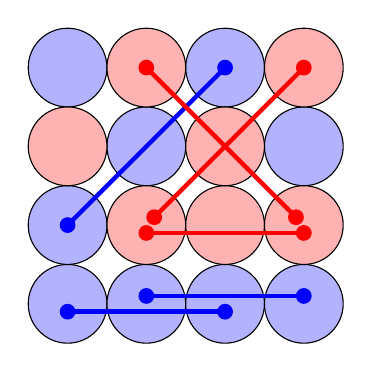
\begin{tikzpicture}
      \foreach \x/\y in {0/0,0/1,0/3,1/0,1/2,2/0,2/3,3/0,3/2} { \draw[fill=blue!30] (\x,\y) circle (0.5cm); }
      \foreach \x/\y in {0/2,1/1,1/3,2/1,2/2,3/1,3/3} { \draw[fill=red!30] (\x,\y) circle (0.5cm); }
      \foreach \x/\y/\a/\b in {0/1/2/3,0/-0.1/2/-0.1,1/0.1/3/0.1} {
        \draw[ultra thick, blue] (\x,\y)--(\a,\b);
        \fill[blue] (\x, \y) circle (0.1cm);
        \fill[blue] (\a, \b) circle (0.1cm);
      }
      \foreach \x/\y/\a/\b in {
        1/3/2.9/1.1,
        1.1/1.1/3/3,
        1/0.9/3/0.9}
      {
        \draw[ultra thick, red] (\x,\y)--(\a,\b);
        \fill[red] (\x, \y) circle (0.1cm);
        \fill[red] (\a, \b) circle (0.1cm);
      }
    \end{tikzpicture}
    \caption{
      In this game on a $4 \times 4$ board, the red player and blue player tie with three points each.
    }
  \end{figure}

\begin{question}
  Which player has a winning strategy?
\end{question}
\begin{related}
  \item What is the score differential under perfect play?
  \item If players cooperate, what is the greatest score differential?
  \item What if this is generalized to a torus or cylinder or M\"obius strip?
  \item What if the game is played with $k$ players or requires $\ell$-in-a-row?
  \item What if the game is played on a triangular grid?
  \item What if the game is played in $d$ dimensions?
\end{related}
\begin{references}
  \item Problem 38.
\end{references}

\end{document}
